\columnbreak

\section{Other Counters}
\label{sec:other-counter}

\subsection{Counter with Unused States}
\label{subsec:counter-with-unused-states}

A circuit with $n$ flip-flops has $2^n$ binary states. There are occasions when a sequential circuit uses fewer than this maximum possible number of states. States that are not used in specifying the sequential circuit are not listed in the state table. In simplifying the input equations, the unused states may be treated as don't-care conditions or may be assigned specific next states. 

It is important to realize that once the circuit is designed and constructed, outside interference during its operation may cause the circuit to enter one of the unused states. In that case, it is necessary to ensure that the circuit eventually goes into one of the valid states so that it can resume normal operation. Otherwise, if the sequential circuit circulates among unused states, there will be no way to bring it back to its intended sequence of state transitions. 

If the unused states are treated as don't-care conditions, then once the circuit is designed, it must be investigated to determine the effect of the unused states. The next state from an unused state can be determined from the analysis of the circuit after it is designed.

Basically, a circuit with $n$ flip-flops has $2^n$ binary states. However, sometimes one may have unused, or leftover states. In the end, we need to consider these states.

\newpage

For example, condsider the following state table and diagram for a counter that repeatedly counts from 0 (000) to 5 (101). What should we put in the table for the two unused states.
\begin{figure}[H]
  \centering
  \begin{minipage}{0.49\linewidth}
      \centering
      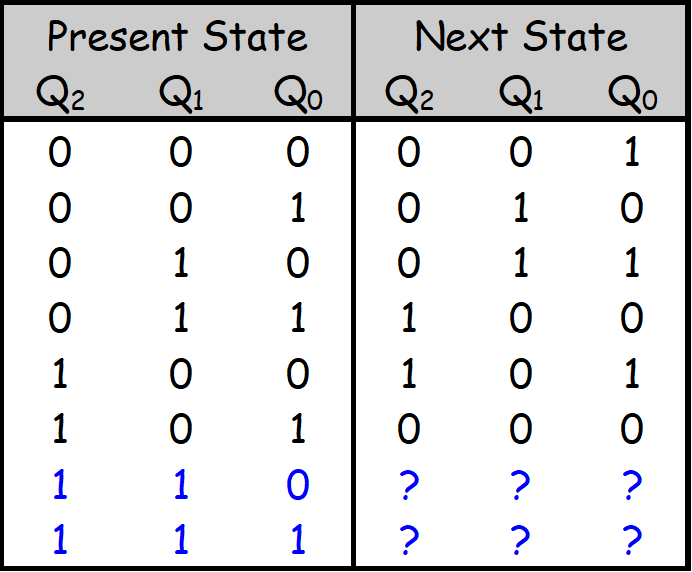
\includegraphics[width=\linewidth]{img/unused-state-table.png}
      \label{fig:unused-state-table}
  \end{minipage}\hfill
  \begin{minipage}{0.49\linewidth}
      \centering
      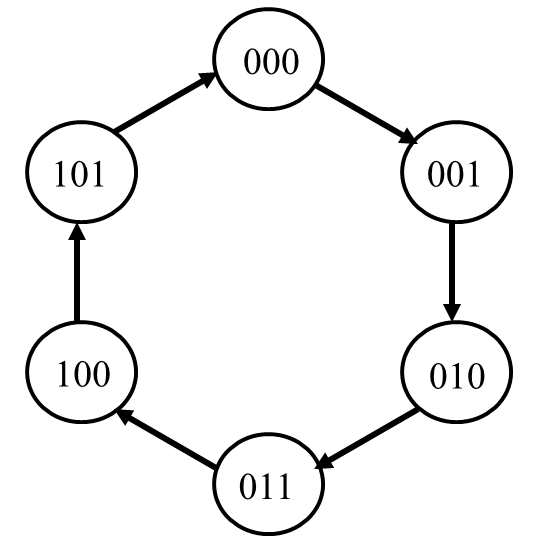
\includegraphics[width=\linewidth]{img/unused-state-diagram.png}
      \label{fig:unused-state-diagram.png}
  \end{minipage}
\end{figure}

To get the simplest possible circuit, you can fill in don't cares for the next states. This will also result in don't cares for the flip-flop inputs, which can simplify the hardware. If the circuit ``somehow'' ends up in one of the unused states (110 or 111), its behavior will depend on exactly what the don't cares were filled in with.

To get the safest possible circuit, you can explicitly fill in next states for the unused states 110 and 111. This guarantees that even if the circuit somehow enters an unused state, it will eventually end up in a valid state. This is called a self-starting counter.

\begin{figure}[H]
  \centering
  \begin{minipage}{0.49\linewidth}
    \centering
    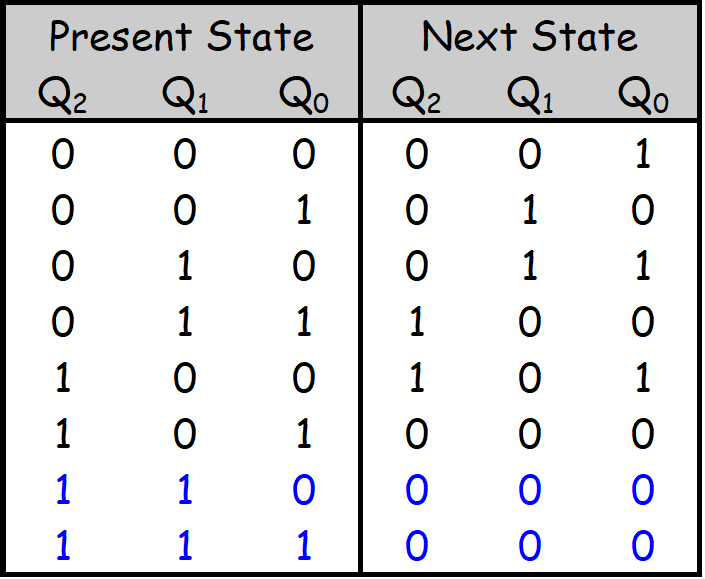
\includegraphics[width=\linewidth]{img/self-starting-counter-table.png}
    \label{fig:self-starting-counter-table.png}
  \end{minipage}\hfill
  \begin{minipage}{0.49\linewidth}
    \centering
    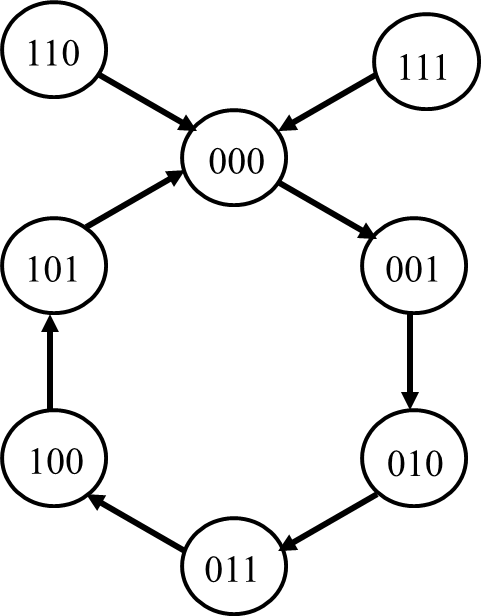
\includegraphics[width=\linewidth]{img/self-starting-counter-diagram.png}
    \label{fig:self-starting-counter-diagram.png.png}
  \end{minipage}
\end{figure}


\subsection{Ring Counter}
\label{subsec:ring-counter}

A \textit{ring counter} is a circular shift register with only one flip-flop being set at any particular time; all others are cleared.

The single bit is shifted from one flip-flop to the next to produce the 
sequence of timing signals. Figure 17(a) shows a four-bit shift register connected as a 8-4-2-1 ring counter.

For an alternative design, the timing signals can be generated by a two-bit counter that goes through four distinct states. The decoder shown in Fig. 17(c) decodes the four states of the counter and generates the required sequence of timing signals.

To generate $2^n$ timing signals, we need either a shift register with $2^n$ flip-flops or an $n$-bit binary counter together with an $n$-to-$2^n$-line decoder.

\setcounter{figure}{16}

\begin{figure}[H]
  \centering
  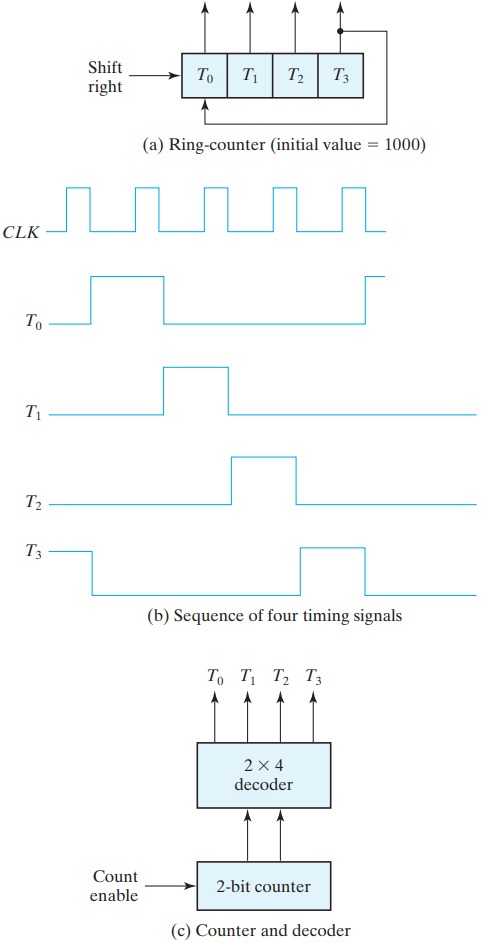
\includegraphics[width=\linewidth]{img/fig-6.17.png}
  \caption{Generation of timing signals}
  \label{fig:6.17}
\end{figure}

It is also possible to generate the timing signals with a combination of 
a shift register and a decoder. That way, the number of flip-flops is less than that in a ring counter, and the decoder requires only two-input gates. This combination is called a \textit{Johnson counter}.

\vspace*{\fill}
\columnbreak

\subsection{Johnson Counter}
\label{subsec:johnson-counter}

A $k$-bit ring counter circulates a single bit among the flip-flops to provide $k$ distinguishable states. The number of states can be doubled if the shift register is connected as a \textit{switch-tail ring counter}. Figure 18(a) shows such a shift register.

\begin{figure}[H]
  \centering
  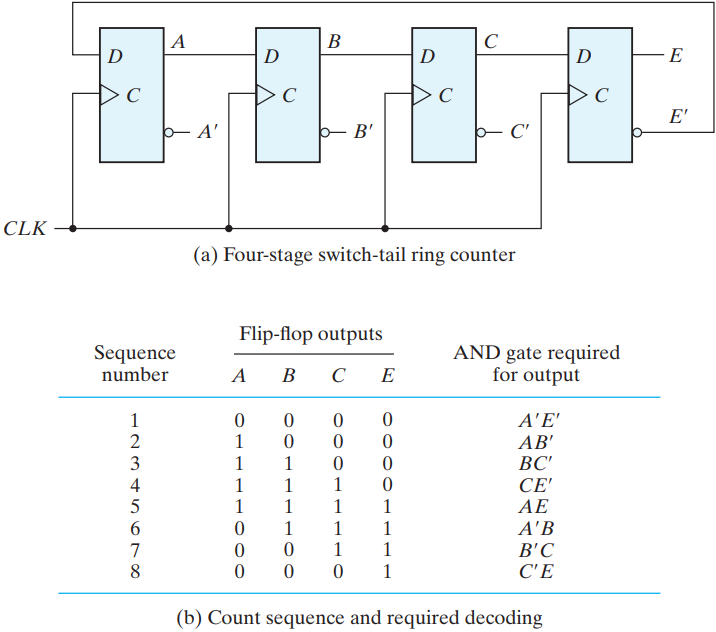
\includegraphics[width=\linewidth]{img/fig-6.18.png}
  \caption{Construction of a Johnson counter}
  \label{fig:6.18}
\end{figure}

Starting from a cleared state, the switch-tail ring counter goes through a sequence of eight states, as listed in Fig. 18(b). In general, a $k$-bit switch-tail ring counter will go through a sequence of $2k$ states.

\vspace*{\fill}
\columnbreak
